\documentclass{vgtc}
% other options: review, preprint, widereview, electronic (for hyperrefs)
% IEEE Vis 2019 does not require anonymous submissions

%% Figures should be in CMYK or Grey scale format, otherwise, colour
%% shifting may occur during the printing process.

%% These few lines make a distinction between latex and pdflatex calls and they
%% bring in essential packages for graphics and font handling.
%% Note that due to the \DeclareGraphicsExtensions{} call it is no longer necessary
%% to provide the the path and extension of a graphics file:
%% \includegraphics{diamondrule} is completely sufficient.
%%
\ifpdf%                                % if we use pdflatex
  \pdfoutput=1\relax                   % create PDFs from pdfLaTeX
  \pdfcompresslevel=9                  % PDF Compression
  \pdfoptionpdfminorversion=7          % create PDF 1.7
  \ExecuteOptions{pdftex}
  \usepackage{graphicx}                % allow us to embed graphics files
  \DeclareGraphicsExtensions{.pdf,.png,.jpg,.jpeg} % for pdflatex we expect .pdf, .png, or .jpg files
\else%                                 % else we use pure latex
  \ExecuteOptions{dvips}
  \usepackage{graphicx}                % allow us to embed graphics files
  \DeclareGraphicsExtensions{.eps}     % for pure latex we expect eps files
\fi%

%% If you are submitting a paper to a conference for review with a double
%% blind reviewing process, please replace the value ``0'' below with your
%% OnlineID. Otherwise, you may safely leave it at ``0''.
\onlineid{0}

%% declare the category of your paper, only shown in review mode
\vgtccategory{Research}

%% allow for this line if you want the electronic option to work properly
\vgtcinsertpkg

%% In preprint mode you may define your own headline.
%\preprinttext{To appear in an IEEE VGTC sponsored conference.}

%% it is recomended to use ``\autoref{sec:bla}'' instead of ``Fig.~\ref{sec:bla}''
\graphicspath{{figures/}{pictures/}{images/}{./}} % where to search for the images

\newcommand\hmmax{0} % http://tex.stackexchange.com/questions/3676
\newcommand\bmmax{0}

\usepackage{float}
\usepackage{mathpartir}
\usepackage{bm}
\usepackage{soul}
\usepackage{xspace}
\usepackage{mathtools}
\usepackage{hyperref}
\usepackage{breakurl}
\usepackage[scaled=0.75]{beramono}
\usepackage{pifont}
\usepackage{framed}
\usepackage{subdepth}
\usepackage{dashundergaps}
\usepackage{listings}
\usepackage{mleftright}
\usepackage{extarrows}
\usepackage{placeins}
\usepackage[a]{esvect}
%\usepackage{upgreek}
\usepackage{colortbl}
\usepackage{tabularx}
\usepackage{multirow}
\usepackage{subcaption}
\usepackage{enumitem}
\usepackage{sfmath}
\usepackage{tikz}
\usetikzlibrary{calc}

\newcommand*{\derivationWidth}{0.6\textwidth}
\input{tex-common/proof-helpers}
\input{tex-common/localref}
\input{tex-common/column-types}
\input{tex-common/relational-override} % no longer need this, but must sync up proofs first


\title{Explorable Data Visualisations}

\author{Roly Perera}
\orcid{0000-0001-9249-9862}
\affiliation{The Alan Turing Institute}
\email{rperera@turing.ac.uk}

\author{Tomas Petricek}
\affiliation{University of Kent}
\affiliation{The Alan Turing Institute}
\email{t.petricek@kent.ac.uk}

\section*{Abstract (500 words):}

Data visualisation is essential to data science and science communication, but
is open to both misinterpretation and misuse: patterns in raw data can be
obscured, statistical assumptions hidden, and effect sizes misrepresented
\cite{weissgerber15}. These concerns can be addressed in part through improved
statistical practices and better plot and chart designs \cite{allen19}, but also
by making visualisations themselves more open and explorable
\cite{dragicevic19}.

Understanding a visualisation requires grasping how it relates to the underlying
data and other visualisations. For example, geoscientists often work with
multiple layered views. To show how these are related, spatial analytics
applications like GeoDa \cite{anselin06} can automatically select the relevant
part of one view as the user changes the selection in a related view, say a
choropleth map. However, this feature is available only if it was specifically
anticipated by the application or library developer; if the geoscientist uses
custom libraries or wants other views linked that the developer did not
consider, they are out of luck.

Our project will deliver a framework for authoring visualisations where support
for linking, between data, code, and visualisations is built in, making this
powerful comprehension feature automatic. To allow us to focus on the needs of
SPF projects working within the Urban Analytics theme, we have assembled a team
with expertise in geocomputation and spatial analytics (Wolf, Malik). This is
complemented with expertise in data visualisation (Bach, Wolf), data provenance
(Cheney, Perera, Malik), and programming languages (Cheney, Perera, Petricek).
The following three tracks will run in parallel, building on a proof-of-concept
also developed within the TPS programme; see
\url{https://www.turing.ac.uk/research/research-projects/data-science-toolkit-explorable-data-visualisations}.

\subsection*{Track 1: Domain use cases}

\paragraph{[Wolf, Malik, Bach, Perera, 0.5 FTE RA]} We will develop a public
repository of substantive geospatial visualisation use cases that demonstrate
the explorability features of our approach to prospective users. This will
ensure that the work in track 1 stays focused on real needs of researchers in
the urban analytics and other geospatial domains.

\subsection*{Track 2: Infrastructure for explorable data visualisations}

\paragraph{[Perera, Petricek, Cheney, Malik, Bach, 0.5 FTE RA]} This will
involve user interface and library design, and new programming language
infrastructure. Driven by our domain use cases (track 1), we will further
develop our toolkit, building on a dynamic program analysis technique developed
by Perera and Cheney \cite{perera12a,ricciotti17}. We will combine the linking
feature with the ability to explore the pipeline of data and visual
transformations that yielded the final artefact, for example by tabbing through
the various intermediate artefacts. We call the resulting explorable
visualisations ``self-explaining'' because they can be explored in situ (say in
an online paper) to reveal how the visualisation was created.

\subsection*{Track 3: Wrattler integration}

\paragraph{[Perera, Petricek, 0.5 FTE RSE]} We will integrate our toolkit with
the Wrattler notebook \cite{petricek18}; this strand of work will also be
supported by the ``Evolving Wrattler into the Turing tools platform" work
package. This is central to our impact strategy and how we connect to other
Turing SPF projects and is discussed in detail later.


\CCScatlist{
  \CCScatTwelve{Human-centered computing}{Visualization}{Visualization systems and tools}{Visualization toolkits};
  \CCScatTwelve{Human-centered computing}{Visualization}{Visualization application domains}{Scientific visualization}
}

%% Copyright enabled by default; disabled by 'review' option or via \nocopyrightspace.
\begin{document}
\maketitle

\section{Introduction}

Data visualisation is essential to data science and science communication, but
is open to both misinterpretation and misuse: patterns in raw data can be
obscured, statistical assumptions hidden, and effect sizes misrepresented
\cite{weissgerber15}. These concerns can be addressed in part through improved
statistical practices and better plot and chart designs \cite{allen19}, but also
by making visualisations themselves more open and explorable
\cite{dragicevic19}.

Understanding a visualisation requires grasping how it relates to the underlying
data and other visualisations. For example, geoscientists often work with
multiple layered views. To show how these are related, spatial analytics
applications like GeoDa \cite{anselin06} can automatically select the relevant
part of one view as the user changes the selection in a related view, say a
choropleth map. However, this feature is available only if it was specifically
anticipated by the application or library developer; if the geoscientist uses
custom libraries or wants other views linked that the developer did not
consider, they are out of luck.

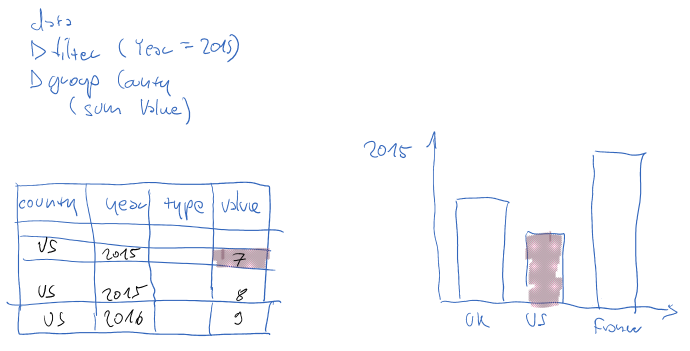
\includegraphics[scale=0.35]{image/chart-fwd}

In this paper we present a framework for authoring visualisations where support
for linking, between data, code, and visualisations is built in, making this
powerful comprehension feature automatic.

% \cite{perera16d,ricciotti17}

\section{Another section}

Our framework provides infrastructure for ``linking'', or multiple-coordinated
views \cite{tobiasz09}, in an application-independent way. The theoretical
foundation of the work is our own prior work on dynamic dependency analysis and
provenance \cite{perera16d, ricciotti17}; in contrast to prior work on
provenance in data visualisation \cite{callahan06}, our approach is much more
fine-grained and is able to associate specific parts of the data or code with
parts of a visualisation in a precise way. While the theoretical technique is
proven, this approach has never been applied to data visualisation before.

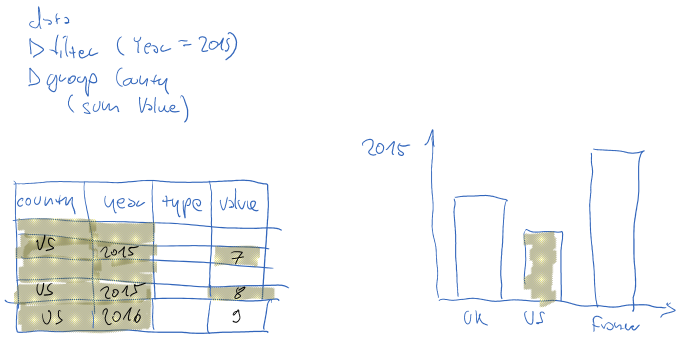
\includegraphics[scale=0.35]{image/chart-bwd}

\section{Conclusions and future work}

There are a number of challenges associated with making our approach practical
and appealing to actual data scientists. A central usability challenge is
visualising these complex relationships between the various parts of a
visualisation and the relevant data and/or visualisation code. This is
essentially a higher-order visualisation problem: visualising information about
the provenance of visualisations. Ideas from temporal data visualisation
\cite{bach16}, data-driven storytelling \cite{bach18}, and ``literate''
visualisation \cite{wood19} may inform our efforts here.

\acknowledgments{}
\bibliographystyle{tex/abbrv-doi}
% Other options: abbrv, abbrv-doi-narrow, abbrv-doi-hyperref, abbrv-doi-hyperref-narrow
\bibliography{../../tex-common/bib}
\end{document}
